\chapter{Regresjonsanalyse}
\label{kap:regresjonsanalyse} % Opprinnelig kapittelnr: 12

\section{Lineære forklaringsmodeller}

Vi er ofte interesserte i å studere sammenhengen mellom en variabel $Y$
og en eller flere andre variable $X_1, X_2, \ldots $.
Her vil $Y$ omtales som {\em den avhengige variable} og de øvrige som   
{\em forklaringsvariable} (av noen misvisende kalt uavhengige variable).
Formålet kan variere: Å se hvordan disse samvarierer med $Y$,
kan forklare $Y$ eller evt. predikere $Y$.


Det vil i mange situasjoner være formålstjenlig å anta 
tilnærmet lineær sammenheng mellom den avhengige og de forklarende
variable:

\[  Y={\beta}_0 + {\beta}_1X_1 + {\beta}_2X_2 + \cdots + {\beta}_rX_r + U \]

\noindent Her er den avhengig variable $Y$ uttrykt som en
lineær funksjon av $r$ for\-klarings\-variable $X_1, X_2, \ldots , X_r$
pluss et restledd $U$, oftest kalt {\em feilleddet}.  Størrelsene
${\beta}_0, {\beta}_1, {\beta}_2, \ldots , {\beta}_r$ er konstanter som
uttrykker betydningen av de respektive forklaringsvariable. $ {\beta}_0$
kalles {\em konstantleddet}, mens $ {\beta}_1, {\beta}_2, \ldots , {\beta}_r$
kalles {\em regresjonskoeffisienter}.  Forklaringsvariablene selv omtales
ofte som {\em regressorer}.
En innføring i lineære forklaringsmodeller med \'{e}n (sikker) 
for\-klarende variabel fins i Kapittel 8.3 og 8.6, og anbefales repetert
før en leser videre.\\



\begin{eksempel}{Avling}
Vi ønsker å studere sammenhengen mellom avling ($Y$) og
forklaringsvariablene  gjødningskvantum ($X_1$), temperatur ($X_2$),
fuktighet ($X_3$) og tid for planting ($X_4$). Aktuell forklaringsmodell er

\[ Y= {\beta}_0 + {\beta}_1X_1 + {\beta}_2X_2 + {\beta}_3X_3 +
                                                   {\beta}_4X_4 + U \]

\noindent Dersom det dreier seg om drivhus vil trolig avling forklares nesten
like godt uten å ta i betraktning tidspunktet for planting.  Det er da
rimelig å
utelate denne forklaringsvariablen, bl.a. for å få en enklere modell.
Andre forklaringsvariable som kan være aktuelle, er veksttid ($X_5$),  
forbrukt kvantum av vern mot skadedyr eller råte ($X_6$), antall
beskjæringer ($X_7$).  Den siste vil antakelig være en 
indikatorvariabel, dvs. ha verdi enten null eller en.
\end {eksempel}

Feilleddet i modellen omfatter den del av den avhengig variable som ikke kan forklares
lineært ved de forklaringsvariable som er benyttet.  Det kan tenkes å
bestå av flere ulike komponenter.  Disse kan være tilfeldig variasjon,
dvs. at forklaringsvariablene ikke entydig bestemmer verdien av den avhengig
variable.  Dette kan skyldes målefeil m.h.t. de variable som inngår,
eller at andre faktorer som ikke er tatt med i mo\-dellen påvirker
resultatet.  Det kan også tenkes at de faktorer som inngår selv innvirker på
feilleddet,  dette er tilfelle dersom den avhengig variable avhenger av
faktorene på en mer komplisert måte enn den som modellen gir uttrykk
for.  I mange situasjoner er en villig til å anta at dette ikke er
tilfelle, i hvert fall ikke i avgjørende grad.
En modell er typisk mest anvendelig dersom feilleddet er lite i forhold til
den forklarende (strukturelle) del.

Med denne antakelsen kan vi gi regresjonskoeffisientene en praktisk 
fortolkning, idet ${\beta}_i$ er den endring av den avhengig variable $Y$
som skyldes at forklaringsvariablen $X_i$ endres med en enhet, mens alle 
andre forkla\-ringsvariable holdes konstant.  Modellen gir da uttrykk for at
den marginale endringen i responsen er den samme for en endring på en
enhet av faktoren, uansett hvilken verdi av faktoren vi tar utgangspunkt i.
Videre uttrykker modellen at de ulike faktorene er additive, og at den
marginale endring av responsen som skyldes endring av en faktor ikke avhenger
av hvilke verdier de andre faktorene har.  Modellen uttrykker med andre ord
at det ikke er samspill mellom faktorene.

Betraktningene ovenfor forutsetter at til hver forklarende faktor $X_i$ svarer en
forklaringsvariabel, nemlig $X_i$ selv.  Imidlertid er antakelsen om 
linearitet ikke så restriktiv som dette.  Det dreier seg om linearitet i
koeffisientene ${\beta}_0, {\beta}_1, {\beta}_2, \ldots , {\beta}_r $, og det
er ingenting i veien for å innføre for\-klaringsvariable som er funksjoner
av de faktorer som inngår.  Eksempelvis kan det tenkes at den marginale
virkningen av en faktor $X_i$ avtar med økende verdi av denne. Det er da
aktuelt å prøve logaritmen til $X_i$ eller kvadratroten av $X_i$ som
forklaringsvariabel, eventuelt i tillegg til $X_i$ selv.  Dersom en og samme
faktor inngår i flere forklaringsvariable, mister vi den konkrete
fortolkning av regresjonskoeffisientene som vi ga ovenfor.  Ved å 
innføre forklaringsvariable som er en funksjon av to eller flere faktorer,
kan vi også få uttrykt visse former for samspill mellom faktorene,
men hvordan dette gjøres vil avhenge av omstendighetene ved hver enkelt
anvendelse.

Lineære forklaringsmodeller er aktuelle fordi de er spesielt enkle å
arbeide med.  I mange situasjoner kan de rettferdiggjøres ut fra den
aktuelle problemstilling, noen ganger kan de argumenteres med at lite er
vunnet ved å bruke en mer realistisk og mer komplisert forklaringsmodell.
I noen situasjoner mangler en forhåndsinnsikt til å argumentere for 
en bestemt forklaringsmodell.  Bruk av lineære modeller kan da
representere et første forsøk på å skaffe en viss innsikt
i situasjonen, med sikte på å lage en rea\-lis\-tisk modell.  Det er da
aktuelt å prøve en rekke forklaringsvariable for å se hvilken
kombinasjon av slike som gir best forklaring.  Kan hende gir ingen lineær
modell tilstrekkelig god forklaring for vårt formål.

Ordet forklaring i forbindelse med bruk av lineære modeller må ikke
tas altfor bokstavelig.  Slike modeller pretenderer å gi en viss innsikt,
ikke nødvendigvis full innsikt.  Den bruk vi kan gjøre av en lineær
for\-klaringsmodell, vil avhenge av de antakelser vi er villige til å 
gjøre om de størrelser som inngår i modellen, samt i hvilken grad
vi ``tror på" modellen.

Dersom vi i en gitt situasjon studerer en avhengig variabel $Y$, og har bestemt
oss for en lineær forklaringsmodell med r forklaringsvariable \\
$X_1,X_2, \ldots , X_r$, vil de koeffisienter ${\beta}_0, {\beta}_1,{\beta}_2,
\ldots , {\beta}_r $ som gir brukbar forklaring som regel være ukjente.
For å få informasjon om de ukjente elementene i modellen, kan vi
observere den avhengig variable for ulike verdikombinasjoner av
forklaringsvariablene.  Et slikt tallmateriale analyseres gjerne ved en
såkalt {\em regresjonsanalyse}.

Formålet med en regresjonsanalyse er i første omgang å fastlegge
regresjonskoeffisientene i henhold til den lineære forklaringsmodellen
på en fornuftig måte.  Utover dette ønsker vi å vurdere den
fastlagte modellens totale forklaringsevne, samt de ulike 
forklaringsvariablenes absolutte og rela\-tive betydning.  Slike betraktninger
kan være til hjelp for eventuell senere bruk av modellen, f.eks. til
prediksjoner eller som grunnlag for beslutninger. 

\section{Minste kvadraters metode}

La oss tenke oss at det foreligger $n$ observasjoner av den avhengig
variable for ulike verdikombinasjoner av forklaringsvariablene, slik

\begin{center}
\begin{tabular}{ccccc}
 $Y_1$&$X_{11}$&$X_{12}$&$\ldots$&$X_{1r}$ \\
 $Y_2$&$X_{21}$&$X_{22}$&$\ldots$&$X_{2r}$ \\
 $\vdots$&$\vdots$&$\vdots$&$   $&$\vdots $ \\
 $Y_n$&$X_{n1}$&$X_{n2}$&$\ldots$&$X_{nr}$ 
\end{tabular}
\end{center}
Her betegner $Y_i$ den $i$'te observasjon av den avhengig variable, mens
$X_{ij}$ er den i'te observasjon av forklaringsvariabel nr. $j$.
For at data overhodet skal være til hjelp, viser det seg at antall
observasjoner $n$ må være minst lik $r+1$. 
I praksis blir som regel regresjonskoeffisientene i en lineær
forklaringsmodell fastlagt ved {\em minste kvadraters metode}, dvs.
${\beta}_0, {\beta}_1, {\beta}_2, \ldots , {\beta}_r $ blir bestemt slik at

\[  \sum_{i=1}^n {[Y_i-({\beta}_0 + {\beta}_1X_{i1} + {\beta}_2X_{i2} +
                 \cdots  + {\beta}_rX_{ir})]}^2     \]

\noindent er minst mulig.  Dette innebærer at forklaringsmodellen blir
fastlagt slik at kvadratsummen av de beregnede feilledd er minst mulig
  \footnote{Metoden er illustrert grafisk i tilfellet med en forklaringsvariabel i 
Kapittel 8.3}, dvs. gir gjennomgående god forklaring for de observerte
data.  De koeffisienter som fastlegges på denne måten betegner vi
$\hat{{\beta}}_0, \hat{{\beta}}_1, \hat{{\beta}}_2, \ldots , \hat{{\beta}}_r.$
Formeluttrykkene er relativt kompliserte, med mindre man innfører
matrisenotasjon. Da er de relativt enkle, og kan lett implementeres i programvare
\footnote{Vektoren av regresjonskoeffisienter kan skrives
 $\hat{\beta} = {(X'X)}^{-1}X'Y$, hvor $X$ er datamatrisen med de forklarende
variable, og der konstantleddet er representert ved en førstekolonne med
enere og $Y$ er kolonnevektoren med $Y_i$'ene.}.
Programvare for slik regresjonsanalyse er idag lett tilgjengelig
for brukere, og disse gir i varierende grad opplysninger for de formål
som er nevnt sist i forrige avsnitt.

I praksis blir ofte resultatet av en regresjonsanalyse presentert slik:

\begin{center} $
 \begin{array}{cccccccccccc}
 \hat{Y}&=&\hat{{\beta}_0}&+&\hat{{\beta}_1}X_1&+&\hat{{\beta}_2}X_2&+&
                           \cdots &+&\hat{{\beta}_r}X_r &(\pm S) \\
        & & &   &(\pm S_1)& &(\pm S_2)& & & &(\pm S_r) & 
 \end{array} $
\end{center}
\noindent Uttrykket uten feilledd kalles den beregnede regresjonsligning, 
der $\hat{Y}$ kalles den beregnede respons.
Dette henger sammen med ønsket om at høyresiden i formelen skal gi
 uttrykk for (anslå) den forventede respons for ulike
 verdi\-kom\-binasjoner $X_1, X_2, \ldots, X_r $ av forklaringsvariablene.
Regresjonsligningen vil i så fall kunne brukes for prediksjonsformål,
og vi kaller derfor $\hat{Y}$ ofte {\em minste kvadraters prediktoren}.

Beregnet respons for de gitte observasjoner blir

\[ \hat{Y_i}=\hat{{\beta}_0}+\hat{{\beta}_1}X_{i1}+\hat{{\beta}_2}X_{i2}+
                           \cdots +\hat{{\beta}_r}X_{ir}  \]

\noindent og forskjellen mellom disse og de tilsvarende observerte responser
(de såkalte residualene) blir $\hat{U_i}=Y_i-\hat{Y_i}$.
Standardavviket $S$ til disse residualene gir uttrykk for hvor god tilpasning
observasjonene har til modellen, og gir også uttrykk for en typisk
prediksjonsfeil dersom ligningen brukes til å predikere responsen
for en ny verdikombinasjon av de forklarende variable.

Størrelsene $S_1, S_2, \ldots , S_r$ ovenfor er standardfeil
knyttet til hver regresjonskoeffisient.  Det er nemlig ikke nok å kjenne
den fastlagte regre\-sjons\-koef\-fisientens absolutte verdi for å vurdere
betydningen av den tilhørende forklaringsvariabel,
idet hver må ses i forhold til sin måleenhet, og viser det seg,
også i forhold til måleenhetene for de andre forklaringsvariablene.
Grovt sagt, jo mindre standardfeilen er i forhold til regresjonskoeffisienten,
desto skarpere konklusjoner kan vi trekke om betydningen
av vedkommende forklaringsvariabel.
Mer presise definisjoner og fortolkninger av størrelsene ovenfor
følger i neste avsnitt.\\


\begin{eksempel}{Fyringsutgifter}
Betrakt eneboliger der parafin er brukt som eneste oppvarming. Årlig
forbruk ($Y$) antas å avhenge av boareal ($X_1$) og lengde på
fyringssesong ($X_2$). Vi har følgende 12 observasjoner fra ulike steder i
landet, med enheter henholdsvis 1000 liter, $m^2$ og måneder.
\begin{center} \addtolength{\tabcolsep}{-0.2\tabcolsep}
\begin{tabular}{|c|rrrrrrrrrrrr|} \hline
 $Y$  &1.2&1.3&1.6&1.0&1.6&1.2&1.1&1.5&1.8&1.0&0.9&1.1 \\
 $X_1$&150&160&100&120&200&125&100&180&200&115&120&150  \\
 $X_2$& 5& 4& 6& 4& 5& 4& 4& 6& 5& 3& 4& 4 \\ \hline
\end{tabular}
\end{center}
Beregning av minste kvadraters prediktoren med tilhørende standardfeil for
koeffisientene og standardavvik til feilleddet, ga resultatet:

\begin{center} $
 \begin{array}{cccccccc}
 \hat{Y}&=&-0.0556&+&0.00337X_1&+&0.1883X_2& (S=0.167)  \\
        & & &   &(\pm 0.00152)& &(\pm 0.0602)&   
 \end{array} $
\end{center}
Data og regresjonsplanet kan illustreres i et tre-dimensjonalt plott.
I to dimensjoner må vi nøye oss med å plotte to variable av gangen,
med nivålinjer for utvalgte verdier av den tredje variablen, se Figur~\ref{fig:2dim_plott}.
\begin{figure}[ht]
\centering
  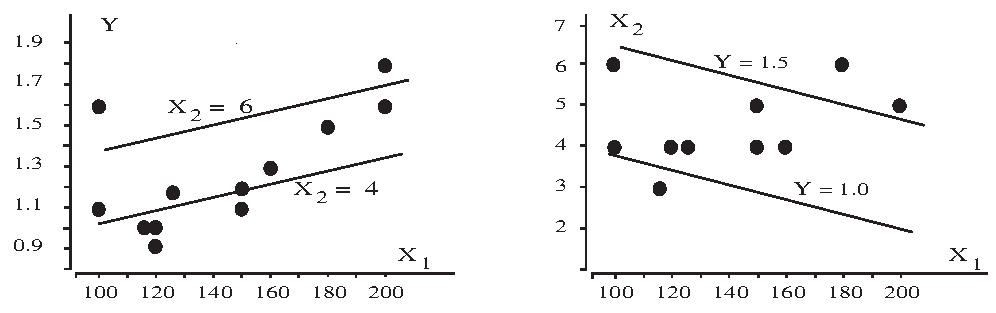
\includegraphics[scale=0.7]{figurer/fig12_1.pdf}
 \caption{To-dimensjonale plott}
	\label{fig:2dim_plott}
\end{figure}

I den beregnede regresjonsligningen er regresjonskoeffisienten til
 $X_1$ (boareal) svært liten, 
men ser vi den i forhold til sin standardfeil, og til måleenheten, er
den en likevel en viktig komponent i forklaringen av fy\-rings\-utgiften, om
enn ikke så viktig som lengden på fyringssesongen. La oss bruke
formelen  til å predikere fyringsutgifter for en enebolig på
100 $m^2$, der  fyringssesongen antas å være 5 måneder. Vi får

\[ \hat{Y}=-0.0556+0.00337\cdot 100+0.1883\cdot 5=1.223 \]

\noindent Den beregnede S=0.167 indikerer at prediksjonsfeilen kan bli stor.
I praksis kan fyringssesongens lengde på et sted variere fra år til
 år, og skal prediksjonen gjøres før sesongen, ved bruk av forventet
 sesong, vil dette gi enda større risiko for prediksjonsfeil. Er det andre
 forklarende variable som kunne være av interesse i dette eksemplet?
\end{eksempel} \\


Et annet mål for tilpasningen til modellen tar utgangspunkt i sammenhengen:

\[ \sum_{i=1}^{n}{(Y_i-\bar{Y})}^2=\sum_{i=1}^{n}{(\hat{Y_i}-\bar{Y})}^2+
                              \sum_{i=1}^{n}{(Y_i-\hat{Y_i})}^2   \]
\noindent som tolkes slik:
\begin{center}
\begin{tabular}{ccc}
Total variasjon &=&variasjon forklart ved $X_1, X_2, \ldots, X_r$ \\
                & &+ uforklart (tilfeldig) variasjon
\end{tabular}
\end{center}
Den såkalte {\em determinasjonskoeffisienten} definert ved

\[ R^2=\frac{\sum{(\hat{Y_i}-\bar{Y})}^2}{\sum{(Y_i-\bar{Y})}^2}=  
              \frac{\mbox{Forklart variasjon}}{\mbox{Total variasjon}} \]

\noindent er et mål  på hvor godt $Y$-observasjonene lar seg
forklare lineært ved $X$-observasjonene. 
Vi ser at $R^2$ er et tall mellom $0$ og $1$, som er lik $1$ hvis og
bare hvis $Y_i ={\hat{Y}}_i$ for alle $i$, dvs. når $Y$-observasjonene er
fullt ut forklart av $X$-observasjonene. I eksemplet ovenfor er
determinasjonskoeffisienten beregnet til 0.72, dvs. hele 72\% av variasjonen
i fyringsutgifter er forklart ved boareal og lengde på fyringssesong.\\

\noindent {\bf Merknad :}  Alternativt kan en beregne 
korrelasjonskoeffisienten, slik den er definert i Kapittel 1 (se også
Kapittel 9.5), mellom $Y$-observasjonene og de tilhørende beregnede 
$\hat{Y}$, dvs.

\[   R=R_{Y\hat{Y}}    \]

\noindent $R$ kalles den {\em multiple korrelasjonskoeffisienten} mellom $Y$ 
og ($X_1, X_2, \ldots, X_r$).  Den har verdi mellom $-1 $ og $+1$, med kvadrat
lik determinasjonskoeffisienten (herav notasjonen ovenfor).  I tilfellet
med en forklarende variabel $X$, viser det seg at $R_{Y\hat{Y}}=R_{YX}$,
dvs. den enkle
korrelasjonskoeffisienten mellom $Y$-observasjonene og $X$-observasjonene.

Som regel er vi interessert i å trekke generelle konklusjoner om de
faktorer som inngår, dvs. konklusjoner som har gyldighet ut over det
foreliggende observasjonsmaterialet.  Vi blir da ledet til å tenke på
det foreliggende materialet som et av mange tenkelige materialer, og det er
da naturlig å vurdere observasjonene i lys av en stokastisk modell.  
Dette gir mulighet for en nærmere vurdering av den analysemetode som 
anvendes, samt en vurdering av usikkerheten ved de konklusjoner som trekkes.

Vi vil nedenfor redegjøre for den standardmodellen som ligger til grunn
for de vanlige regresjonsprogrammer, og se på hvordan de opplysninger
slike programmer vanligvis gir, kan tolkes i lys av standardmodellen.  
Videre vil vi diskutere de enkelte forutsetningene i standardmodellen og
antyde ulike omstendigheter der disse kan være urealistiske.  En vanlig
regresjonsanalyse basert på minste kvadraters metode kan da lett lede
til feiltolkninger av observasjonene, men i slike situasjoner kan en ofte
gjøre bruk av alternative regresjonsmodeller og analysemetoder.  


\section {Standardregresjonsmodellen}

I den linære forklaringsmodellen vil vi gjøre følgende 
tilleggantakelser:

Vi vil oppfatte forklaringsvariablene $X_1, X_2,\ldots , X_r$ som sikre
variable, dvs. ikke underlagt tilfeldigheter
\footnote {For å markere dette
brukes ofte små bokstaver $x_1, x_2, \ldots, x_r$.}.  Feilleddet $U$ vil
vi imidlertid oppfatte som en stokastisk variabel som uttrykker tilfeldig
variasjon.  Mer konkret vil vi anta at $U$ har forventning null og en
bestemt ukjent varians ${\sigma}^2$.  Dette innebærer at $Y$ også blir en
stokastisk variabel.  Forventningen til $Y$ blir

\[  EY= {\beta}_0 + {\beta}_1X_1 + {\beta}_2X_2 + \cdots + {\beta}_rX_r \]

\noindent og dens varians ${\sigma}^2$.
 Her blir altså ${\beta}_0, {\beta}_1, {\beta}_2,\ldots, {\beta}_r $
og ${\sigma}^2$ ukjente parametre som vi ønsker nærmere kunnskap om.

For dette formål foretar vi $n$ gjentatte observasjoner av den avhengig
variable og de tilhørende forklaringsvariable.  Vi vil anta at de $n$
feilleddene er uavhengige av hverandre, som er ekvivalent med å anta
at de avhengig variable er innbyrdes uavhengige.  Med den notasjon vi har brukt før kan vi oppsummere modellen slik:

\begin{center} \framebox[10cm]{\begin{minipage}{9cm}\rule{0cm}{0.5cm}
{\bf Standardregresjonsmodellen :} \\
Gitt observasjoner ($Y_i,X_{i1},X_{i2}, \ldots, X_{ir})\;\;\; i=1,2, \ldots, n$ der

\[ Y_i= {\beta}_0 + {\beta}_1X_{i1} + {\beta}_2X_{i2} + \cdots
              + {\beta}_rX_{ir}+U_i \]

hvor $U_1,U_2, \ldots, U_n$ er uavhengige stokastiske variable med 
forventning null og varians ${\sigma}^2$.\\
  \end{minipage}} \end{center}

\noindent Vi vil nedenfor vurdere konsekvensen av enda en antakelse, nemlig at
feilleddene er normalfordelte, i vår modell betyr dette at de avhengige
variable selv er normalfordelte.  Denne modellen generaliserer den enkle
regresjonsmodellen i Kapittel 8.3 til situasjoner med mer enn en 
forklaringsvariabel.  Notasjonen avviker noe fra den vi brukte der, idet vi
her bruker den notasjon som er mest vanlig ved beskrivelse av flere variable.

La $ \hat{{\beta}_0},\hat{{\beta}_1}, \ldots,\hat{{\beta}_r}$ være minste
kvadraters
estimatorene for parametrene ${\beta}_0,{\beta}_1, \ldots, {\beta}_r$.  For
å sikre at disse er veldefinerte og lar seg beregne, trengs en teknisk
antakelse, nemlig at ingen forklaringsvariabel er overflødig ved at
dens verdi kan skrives som en lineær funksjon av andre forklaringsvariable.
I motsatt fall har vi såkalt {\em multikolinearitet} som medfører at
regresjonskoeffisientene ikke er entydig bestemt.  Nesten
multikolinearitet er også lite ønskelig da dette gir både
beregningsmessige problemer og stor usikkerhet m.h.t. konklusjoner. 

Under forutsetningene i standardregresjonsmodellen blir minste kvad\-raters
estimatorene $\hat{{\beta}_0},\hat{{\beta}_1},\ldots ,\hat{{\beta}_r}$
forventningsrette for sine respektive para\-metre, dvs.

\[   E{\hat{\beta}}_j={\beta}_j  \mbox{\ \ \ \ } j=0,1, \ldots,r. \]

\noindent Deres respektive varianser kan beregnes, og de har følgende form

\[ var{\hat{\beta}}_j=\frac{{\sigma}^2}{M_j} \mbox{\ \ \ \ } j=0,1,\ldots,r.\]

\noindent der $M_j$ er en funksjon av de observerte verdier av alle
forklaringsvariablene.  I tilfellet med en forklaringsvariabel er formelen
for variansen til regre\-sjons\-koeffi\-sienten gitt i Kapittel 8.3, men allerede
for to forklaringsvariable er formlene for beregning av $M_j$'ene nokså
kompliserte med mindre man tar i bruk matrisenotasjon.
Det kan imidlertid vises at
\[ M_j = (1-R_j^2) \cdot \sum_{i=1}^{n} (X_{ij}-\bar{X}_j)^2    \]
der $R_j^2$ er determinasjonskoeffisienten ved en regresjon med $X_j$ som
avhengig variabel og de øvrige $X$'er som forklarende variable.
Vi ser at $var{\hat{\beta}}_j$ øker med $R_j^2$ og multikolinearitet 
er problematisk dersom $R_j^2 > 0.9$.

Minste kvadraters estimatorene viser seg å være lineære 
funksjoner av de observerte avhengig variable.  Dette betyr at dersom vi er
villig til å anta at observasjonene er normalfordelte, så er også
disse estimatorene normalfordelte med forventning og varians gitt ovenfor.  
Dersom observasjonene ikke antas normalfordelte, vil estimatorene likevel
være tilnærmet normalfordelte under visse forutsetninger, bl.a. må
hverken $n$ eller $M_j$'ene være for små.

Residualene $\hat{U}_i$ kan oppfattes som et
forsøk på å anslå virkelige feilledd $U_i$, og kan brukes til
 å estimere variansene til feilleddene. Det kan vises at

\[ S^2=\frac{1}{n-(r+1)} \sum_{i=1}^{n} {\hat{U}}_i^2    \]

\noindent er en forventningsrett estimator for ${\sigma}^2$.  Merk at $r+1$ er
 antall ukjente
parametre i regresjonsuttrykket, sml. tilfellet med en forklaringsvariabel.
En rimelig estimator for variansen til hver enkelt regresjonskoeffisient
får vi ved å erstatte ${\sigma}^2$ med $S^2$ i formlene for
variansene gitt ovenfor.

Når en skal vurdere betydningen av en rekke estimerte 
regresjons\-koef\-fisienter, trengs et mål for den usikkerhet som må
tillegges hver av dem.  På bakgrunn av opplysningene ovenfor er det
naturlig å betrakte estimert standardavvik, dvs.
$S_j=S({\hat{\beta}}_j)=S/\sqrt{M_j}$.
Brukes vår vanlige rappor\-terings\-metode oppgis

\[{\hat{\beta}}_j \; \; \pm \; \; S({\hat{\beta}}_j)\mbox{\ \ \ \ }j=1,2,\ldots, r. \] 

\noindent Det er vanskelig å gi presise utsagn om estimeringsfeilen uten
å anta at observasjonene er normalfordelte.  I dette tilfellet er nemlig 

\[  T_j=\frac{{\hat{\beta}}_j-{\beta}_j}{S({\hat{\beta}}_j)}    \] 


\noindent $t$-fordelt med $n-r-1$ frihetsgrader. Ved hjelp av en $t$-tabell kan
vi defor gi eksakte sannsynlighetsutsagn om estimeringsfeilen, f.eks. i form
av konfidensintervaller for regresjonskoeffisientene.

Det kan også være av interesse å teste hypoteser om 
regresjonskoeffisientene. Mest aktuell er kanskje $H_0:{\beta}_j=0$, dvs. at
forklaringsvariablen $X_j$ overhodet ikke påvirker den avhengig variable.
Som testobservator kan vi bruke $T_j$ ovenfor, hvor vi har erstattet ${\beta}_j
$ med null.  Under forutsetning av normalfordelte observasjoner vil denne 
testobservator, dersom nullhypotesen er riktig, være $t$-fordelt med
$n-r-1$ frihetsgrader.  Vi er dermed i stand til å lage tester med et
gitt signifikansnivå, eventuelt beregne $P$-verdier for det observerte
resultat.

Vi ser at for å gjøre de betraktninger som er skissert ovenfor, er det
nok å kjenne til de estimerte regresjonskoeffisienter $ \hat{{\beta}_1},
\hat{{\beta}_2},\ldots, \hat{{\beta}_r}$ og de tilhørende estimerte
standardavvik $S_1,S_2,\ldots,S_r$.  I tillegg til dette gir 
regresjonsprogrammer vanligvis også $T_1, T_2, \ldots, T_r $ og $S$
(evt.$S^2$), og i noen tilfeller skrives også ut residualene.

Standardregresjonsmodellen gir også muligheter for å vurdere 
usikkerheten som ligger i å bruke den beregnede regresjonsligning som
prediktor.  Feilmarginer for prediksjonsfeilen blir gjerne konstruert med
utgangspunkt i estimatet $S$ for standardavviket til feilleddet.  Grovt sagt
vil prediksjonsfeil av størrelse opp til \'{e}n gang dette standardavviket
kunne inntreffe relativt ofte, feil omkring to ganger standardavviket
inntreffer også en gang i blant, mens prediksjonsfeil på mer enn tre
ganger standardavviket vil inntreffe svært sjelden.  Dersom antall
observasjoner $n$ er relativt stort i forhold til antall forklaringsvariable,
vil vanligvis 68\% - 95\% regelen gi en viss pekepinn, men ellers er denne
nok noe optimistisk.  Dersom observasjonene er normalfordelte, er det mulig
å lage mer presise sannsynlighetsutsagn om prediksjonsfeilen med 
utgangspunkt i $t$-tabellen med $n-r-1$ frihetsgrader.

Standardregresjonsmodellen generaliserer teorien i Kapittel 8.3 fra en til
flere forklaringsvariable.  De metoder som er foreslått har tilsvarende
optimale egenskaper som i tilfellet med en forklaringsvariabel, og vil skal
ikke gå i detalj her.


\section {Diskusjon}
Vi vil nå drøfte hver av antakelsene i standardmodellen med sikte
på å skape en viss forståelse for de muligheter og
begrensninger som er knyttet til regresjonsanalyse:

Antakelsen om at forklaringsvariablene er sikre variable vil først og
fremst være aktuell i situasjoner der det utføres et eksperiment
med en respons som observeres for ulike verdikombinasjoner av en eller flere
for\-kla\-rings\-variable (stimuli, innsatsfaktorer e.l.) valgt av den som 
utfører eks\-peri\-men\-tet.  Vi kaller dette et eksperiment av 
stimulus-respons typen.  Som eksempel ta et drivhuseksperiment  der avling
observeres for ulike kombinasjoner av gjødningskvantum, temperatur, 
fuktighet etc.

Antakelsen om at feilleddene er uavhengige med samme varians kan ofte
rettferdiggjøres ved at de gjentatte observasjonene av responsen skjer
uavhengig av hverandre for de ulike verdikombinasjoner av 
forkla\-rings\-varia\-blene, men slik at eksperimentbetingelsene ellers er de 
samme fra gang til gang.  Dette er et eksempel på et såkalt (delvis)
kontrollert eksperiment.  Feilleddet kan da tenkes å omfatte usikkerhet
som skyldes målefeil og/eller tilfeldig variasjon som skyldes de faktorer
som ligger utenfor vår kontroll.  Det er imidlertid grunn til å tenke
over antakelsen om samme varians for de ulike verdikombinasjoner.  
Eksempelvis kan det tenkes at visse kombinasjoner av temperatur og fuktighet
gjør plantene mer mottakelige for visse sykdommer enn andre, med økt
risiko for sterk reduksjon av avlingen som ikke er til stede ellers.

Antakelsen om at feilleddet er normalfordelt, som er nødvendig for eksakte
sannsynlighetsutsagn basert på opplysningene fra regresjonsanalysen, vil
kunne brukes dersom vi enten har empirisk erfaring som støtter antakelsen,
eller mener at feilleddet skyldes en rekke uavhengige faktorer som hver 
bidrar lite.

Antakelsen om at forventet respons er en lineær funksjon av 
forklaringsvariablene er alltid åpen for diskusjon.  Selv om dette ikke
er rimelig for alle verdikombinasjoner av forklaringsvariablene, eksempelvis
for ekstremt høye gjødningskvanta og ekstremt høye og lave 
temperaturer, kan det være en rimelig antakelse innenfor det 
verdiområde  vi regner med å gjøre  bruk av modellen og de 
konklusjoner som følger av denne.  Vi har tidligere antydet at
linearitet ikke er så restriktivt som det kan se ut for, idet vi kan
betrakte funksjoner av faktorene som forklaringsvariable.  I mange 
situasjoner er det ikke rimelig å anta at observert respons selv kan
beskrives med en lineær forklaringsmodell.  Typisk eksempler er en
rekke såkalte vekstmodeller.  For slike situasjoner kan det tenkes
alternative forklaringsmodeller som ikke er lineære.  Disse blir straks
vanskeligere å arbeide med både matematisk og fortolkningsmessig.
I noen situasjoner kan det imidlertid tenkes at en størrelse avledet av
responsen kan la seg forklare lineært.  I så fall brukes denne som
avhengig variabel istedenfor responsen selv.  Ved eksponensiell vekst er det
eksempelvis aktuelt å betrakte logaritmen til responsen som avhengig
variabel.  Det vil føre for langt å gå i detalj her, fordi de
muligheter som byr seg vil avhenge av omstendighetene (se Oppgave~6 og~7).

Mindre avvik fra forutsetningene i standardmodellen vil neppe ha
konsekvenser for eventuelle konklusjoner som trekkes på grunnlag av
denne.  Mindre avvik fra linearitet fanges opp av feilleddet som økt 
usikkerhet i tillegg til de rent tilfeldige variasjoner.  Observasjon av
forklaringsvariablene kan ofte innebære en viss usikkerhet i form av
målefeil, men så lenge disse er små i forhold til 
usikkerheten i feilleddet, spiller det liten rolle om de i modellen blir
betraktet som sikre variable.  Mindre ulikheter i variansen fra
observasjon til observasjon spiller også liten rolle.  Det samme gjelder
mindre avvik fra normalitet, dersom vi velger å bruke denne antakelsen.

Større avvik fra forutsetningene vil det ofte være mulig å
avsløre når observasjonene analyseres.  Mye kan læres ved å
studere residualene, dvs. differensen mellom observert respons og 
``beregnet forventet respons" ut fra modellen.  Ifølge modellen bør
disse variere tilfeldig omkring null.  De kan imidlertid vise seg å
ha særtrekk som gjør det nødvendig å modifisere modellen. 
Eksempelvis bør det faktum at en eller flere residualer er svært
store i tallverdi vies spesiell oppmerksomhet, da modellen har gitt 
dårlig forklaring av disse observasjonene.  Vurderer vi residualene 
i forhold til estimert standardavvik for feilleddet, får vi en pekepinn
på om avvikene kan skyldes tilfeldigheter.  Dersom dette ikke synes
rimelig, bør en vurdere en rekke muligheter:  Avvikene kan skyldes at
sannsynlighetsfordelingen til feilleddet er ikke-normal med betydelig 
risiko for ``ville" observasjoner.  Det er utviklet metoder til å teste
antakelsen om normalitet på grunnlag av residualene.  Dersom det er
flere avvikende residualer bør en vurdere om disse har visse fellestrekk,
eksempelvis om de kan forklares ved en variabel som vi har utelatt i 
modellen, f.eks. en variabel som er utenfor vår kontroll.  Dersom de
avvikende responsene er observert etter hverandre i tid, kan en stille 
spørsmålstegn ved antakelsen om uavhengige observasjoner.

Ovenfor har tankene kretset om et (delvis) kontrollert eksperiment av
stimulus-respons typen.  Ved et godt planlagt eksperiment av denne typen er
mulighetene best for å realisere antakelsene i standardmodellen.  I
mange situasjoner er det imidlertid ikke mulig å ha full kontroll over
alle aktuelle forklaringsvariable og tildele disse sikre verdier.  Ofte må
man nøye seg med å observere forklaringsvariablene som del av
eksperimentet selv.  Som eksempel ta et frilandseksperiment hvor riktignok
gjødning kan tilsettes i gitte kvanta, mens temperatur og nedbør ikke
kan det.  Disse forkla\-rings\-variablene kan ikke lenger oppfattes som sikre
variable, men må isteden oppfattes som stokastiske variable med verdier
som realiseres i løpet av eksperimentet, eksempelvis gjennomsnittsverdier
for vekstperioden.  I samfunnsvitenskapene vil det som regel alltid være
slik at viktige forkla\-rings\-variable er utenfor vår kontroll.  Siden deres
verdier ikke er gitt på forhånd, må disse representeres ved
stokastiske variable i eventuell forkla\-rings\-modell.

Den lineære forklaringsmodellen er fortsatt aktuell, men som vi ser er
vi nå utenfor rammen av standardregresjonsmodellen.  Heldigvis viser det
seg mange av de teoretiske resultater som er utviklet for 
standard\-mo\-dellen også gjelder i situasjonen med stokastiske
forklaringsvariable under en viktig, men ofte oversett forutsetning, nemlig
at forklaringsvariablene er uavhengige av feilleddet.  Minste kvadraters
estimatorene for regresjons\-koeffisientene er fortsatt forventningsrette.
Deres varianser er imidlertid noe mer kompliserte enn for
standardmodellen.  Det kan imidlertid gis teoretiske argumenter for at
rapportering av usikkerheten ved estimeringen bør skje betinget gitt
de observerte verdier av forklaringsvariablene, dvs. på samme måten
som i det sikre tilfellet.  Ved testing brukes også de samme metoder som
for standardmodellen, idet man kan vise at testobservatorene, under
normalitet, har den samme sannsynlighetsfordeling som i det sikre tilfellet.
I praksis vil derfor dataanalysen kunne foregå akkurat på samme 
måte i de to situasjonene, den eneste forskjell er at vi i tilfellet
med et kontrollert eksperiment kan velge bestemte verdikombinasjoner av
forklaringsvariablene med hensikt for å redusere usikkerheten, i
motsetning til å måtte ta dem som de kommer.\\

\begin{eksempel}{Avling og vær}
En bonde har de siste åtte årene dyrket samme vekst.  Han har hvert
år notert seg avlingen i kilo pr.~arealenhet, samt nedbør i
centimeter og gjennomsnittstemperatur i vekstperioden.  Han har hele tiden
brukt samme kvantum av en bestemt gjødning, og regner også med at
jorden stort sett var av samme kvalitet og fikk samme kultivering.  Anta
at resultatene ble:

\begin{center}
 \begin{tabular}{lcccccccc}
Avling($Y$):        &  70  &  60  &  80  &  80  &  90  &  60  &  70 &  50 \\
Nedbør ($X_1$):  &  10  &  20  &  25  &  20  &  15  &  15  &  30 &  25 \\
Temperatur ($X_2$): &  25  &  18  &  22  &  22  &  25  &  18  &  16 &  16 \\
\end{tabular}
\end{center}

\noindent Vi vil gjøre bruk av en regresjonsmodell
 $ Y={\beta}_0 + {\beta}_1X_1+{\beta}_2X_2 + U $
 der vi antar at feilleddet er tilfeldig variasjon som
skyldes en rekke uavhengige faktorer som ikke er korrelert hverken med
temperatur eller nedbør.  Observasjonene gir oss følgende estimerte
regresjonsuttrykk 

\[  \begin{array}{ccccccc}
       \hat{Y}&=&-39.2&+&1.26X_1&+&4.15X_2       \\
              & &     & &(\pm 0.55)& &(\pm 0.96)
    \end{array} \]

\noindent Determinasjonskoeffisienten er beregnet til $0.79$, slik at den
 lineære modellen har gitt god forklaring.

Vi ser begge regresjonskoeffisientene er positive, og vurdert i forhold til
de estimerte standardavvik er begge signifikant forskjellig fra null.  Dette
samsvarer med de tanker bonden hadde på forhånd, for en gitt 
tempe\-ratur vil avlingen gjennomgående øke med nedbøren, for en gitt
nedbør vil avlingen gjennomgående øke med temperaturen,
dvs. egenvirkningen av begge forklaringsvariablene er positiv.  Dersom denne
regresjonsligningen brukes til prediksjon vil, dersom vi observerer en
nedbør på 20 cm og gjennomsnittstemperatur på 20 grader C, predikert
avling bli 68.9 kilo pr.~arealenhet.  Vi har også beregnet 
korrelasjonskoeffisientene

\[  R_{YX_1}=-0.17 \; \; \; \; R_{YX_2}=0.76  \; \;\; \;  R_{X_1X_2}=-0.67  \]

\noindent Hvordan kan det ha seg at den første er negativ mens den
 tilsvarende regresjonskoeffisienten er positiv?
\end{eksempel}

I situasjoner der en eller flere stokastiske forklaringsvariable er 
korrelert med feilleddet bryter teorien ovenfor sammen, og vanlig 
regresjonsanalyse basert på minste kvadraters metode kan lede til
alvorlige feiltolkninger.\\


\begin{eksempel}{Avling og vær}
La situasjonen være som beskrevet i forrige eksempel.  Anta at det
ikke foreligger opplysninger om temperaturen, og nedbør ($X_1$) blir 
brukt som eneste forklaringsvariabel.  Observasjonsmaterialet ovenfor gir
da følgende regresjonsuttrykk

\[  \begin{array}{ccccc}
        \hat{Y}&=&76.6&-&0.33X_1       \\
               & &    & &(\pm 0.81)
 \end{array} \]
Vi ser at regresjonskoeffisienten er negativ, men så pass liten i
forhold til standardavviket at vi ledes til å konkludere at nedbør
er uten betydning for avlingen.  Sett i forhold til resultatet i Eksempel
3, hvor konklusjonen var at avlingen økte med økende nedbør virker
dette forvirrende.  Følgende betraktninger kan imidlertid bidra til å
forstå det som har skjedd:  Vår forklaringsmodell er $ Y={\beta}_0 +
{\beta}_1X_1 + U $, der ${\beta}_1 $ skal gi uttrykk for den systematiske
endringen i avling som skyldes en økning i nedbør på en cm når
alle andre faktorer ellers er de samme, og $U$ er tilfeldig variasjon.  I den
grad temperatur ($X_2$) har betydning for avlingen, vil det komme til uttrykk
i feilleddet som tilfeldig variasjon fra år til år.  Nå viser
nedbør og temperatur erfaringsmessig negativ samvariasjon, mye nedbør
som regel sammen med lave temperaturer.  Dette betyr at $X_1$ og $U$
sannsynligvis ikke er uavhengige, men vil ha negativ samvariasjon.  La oss
illustrere mulige konsekvenser av dette med Figur~\ref{fig:korrelerte}.
\end{eksempel}

\begin{figure}[ht]
\centering
  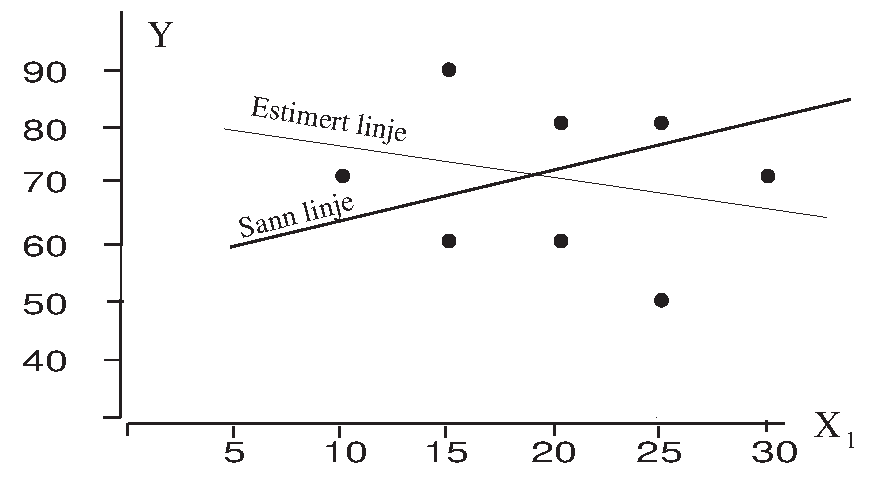
\includegraphics[scale=0.7]{figurer/fig12_2.pdf}
 \caption{Korrelerte feilledd}
	\label{fig:korrelerte}
\end{figure}

I figuren er inntegnet den ``sanne" regresjonslinjen som er stigende med 
$X_1$, dvs. ${\beta}_1$ positiv.  På grunn av de forhold som er nevnt
ovenfor, vil feilleddene i år med lav (høy) nedbør være
gjennomgående positive (negative), dvs. som på figuren.  Vi ser
at enhver estimeringsmetode basert på tilpasning av en rett linje i
spredningsdiagrammet, slik som minste kvadraters metode, vil feilestimere
regresjonslinjen.  I dette tilfellet vil ${\beta}_1$ bli underestimert,
noe som forklarer resultatet ovenfor.  Den estimerte linjen gir altså
ikke et korrekt bilde av egenvirkningen av $X_1$ som forklaringsvariabel,
men har istedenfor gitt oss et visst inntrykk av virkningen av $X_1$ i
samspill med andre faktorer, her trolig i første rekke temperatur.
Den linje som er beregnet gir altså uttrykk for at totalvirkningen av
en økning av nedbøren er omtrent null, eller svakt negativ.  I lys
av resultatene i Eksempel 3 hvor vi fant at egenvirkningen av både 
nedbør og temperatur var positiv, kan dette tolkes dithen at nedbør
utover det normale et bestemt år har en positiv direkte effekt på
avlingen, men denne blir mer enn oppveiet av en negativ indirekte effekt
som skyldes at mye nedbør gjerne følges av lave temperaturer.  Den
regresjonslinje som er beregnet her er derfor fortsatt aktuell dersom vi
neste år skal predikere avlingen for en gitt nedbørmengde, uten 
kjennskap til temperaturen, eksempelvis for nedbør på 20 cm
predikerer vi avlingen 70.0 kilo pr.~arealenhet.

Situasjoner der forklaringsvariablene og feilleddet er korrelerte kan dukke
opp i mange sammenhenger og det kan være lett å overse dette.  Det
som spesielt gjør situasjonen vanskelig, er at vi ofte ikke er i stand til 
å avgjøre dette ut fra observasjonene selv, f.eks. ved studium av
residualene.  Vi har tilsynelatende fått god tilpasning, men er likevel
blitt lurt. Dette kan ofte være et problem i mange samfunnsfaglige
undersøkelser.

  En annen omstendighet som kan lede til feilkonklusjoner
har vi dersom feilleddene i regresjonsmodellen ikke er innbyrdes uavhengige.
Dette vil ofte kunne være tilfelle i situasjoner der observasjonene av
responsen er tatt ved suksessive tidspunkter, slik at det er mulighet for 
en viss tidsavhengighet.  Vi vil ta opp problemer av denne art i neste 
kapittel om tidsrekker.



\section{Anvendelser}

Siden regresjonsanalyse trolig er den mest brukte (og misbrukte) statistiske
inferensmetode i praksis, vil vi ta for oss enkelte detaljer ved analysen av
et tallmateriale med flere forklarende variable.\\

\begin{eksempel}{Studieprestasjoner}
For et tilfeldig utvalg på 39 ferdigutdannede siviløkonomer fra et 
årskull (1984) foreligger registrering av følgende variable:

\begin{center}
\begin{tabular}{ccl}
 $X_1$ &:& Kjønn (0=Mann, 1 = Kvinne)  \\
 $X_2$ &:& Alder (Antall år ved opptak) \\
 $X_3$ &:& Praksis (Antall år før opptak) \\
 $X_4$ &:& Skolepoeng fra videregående skole (75 = 5 i snitt) \\
 $X_5$ &:& Norsk\-karakter \\
 $X_6$ &:& Matematikk\-karakter \\
 $X_7$ &:& Antall år med matematikk \\
 $X_8$ &:& Studieretning (1=Naturfaglig, 2 = Samfunnsfaglig, \\
       & & \mbox{\ \ \ \ \ \ \ \ \ }3 = Språklig, 4 = Handel og kontor) \\
   $Y$ &:& Gjennomsnittskarakteren til siviløkonomeksamen \\
       & &(karakterskala fra 0 til 9, med 9 som topp). 
\end{tabular}
\end{center}

\noindent Disse opplysningene er lagt inn på datafil 'eks12.5' med 39
 linjer (en for hver student) og 9 kolonnefelter (ett for hver variabel). I den
følgende analysen søker en å forklare ``responsvariablen" $Y$ ved
$X_1,X_2,\ldots , X_7$. $X_8$ holdes foreløbig utenfor av grunner vi kommer
 tilbake til.

\begin{center} \framebox[11cm]{\begin{minipage}{10cm}\rule{0cm}{0.5cm} \tt
\noindent >> READ 'eks12.5' Y X1-X8 \\
\begin{tabular}{rrrrrrrrrr}
  Row &  Y & X1  &  X2 &  X3 &  X4  &  X5  &  X6 & X7 & X8   \\
    1 & 5.1&  0  &  22 &   2 &  71  & 4.0  & 5.0 &  3 &  1   \\  
    2 & 3.6&  0  &  21 &   1 &  67  & 4.0  & 4.0 &  3 &  1   \\
    3 & 4.9&  0  &  21 &   1 &  73  & 4.0  & 5.0 &  1 &  2   \\
    4 & 6.6&  0  &  20 &   1 &  81  & 5.0  & 6.0 &  2 &  2  
\end{tabular} \\
   .  .  . 39 ROWS READ \\ 
\addtolength{\tabcolsep}{-0.6\tabcolsep}
 >> REGRESS Y on X1-X7 \\
\begin{tabular}{ccccccccccc}
  Y &=& 2.49&-&0.838 X1&-&0.063 X2&-&0.553 X3&-&0.0162 X4  \\
    & &     &+&0.290 X5&+&0.884 X6&+&0.159 X7& &(S=0.787)  \\
\end{tabular} \\
\addtolength{\tabcolsep}{0.6\tabcolsep}
\begin{tabular}{rrrr}
          &             &  St. Dev.  & T-ratio =\\
 Variable & Coefficient &   of coef. &  coef/s.d.\\
          &       2.487 &     5.860  &      0.42 \\
       X1 &     -0.8377 &    0.3222  &     -2.60 \\
       X2 &     -0.0633 &    0.1968  &     -0.32 \\
       X3 &     -0.5533 &    0.3732  &     -1.48 \\
       X4 &     -0.0163 &    0.0645  &     -0.25 \\
       X5 &      0.2899 &    0.3981  &      0.73 \\
       X6 &      0.8844 &    0.3213  &      2.75 \\
       X7 &      0.1591 &    0.1858  &      0.86
 \end{tabular} \\
Degrees of freedom for T-test = 31 \\
R-squared = 49.9 \% (adjusted for d.f. 38.6 \%)\\
 \end{minipage}} \end{center}


\noindent Utskriften gir

\[ \hat{Y}=\hat{{\beta}_0}+\hat{{\beta}_1}X_1+ \hat{{\beta}_2}X_2 +
                 \cdots + \hat{{\beta}_7}X_7   \]

\noindent med $\hat{{\beta}_j}$, $S(\hat{{\beta}_j})$ og
 $T = \hat{{\beta}_j}/S(\hat{{\beta}_j})$ i egne kolonner.
Den siste gir mulighet for å teste
hypotesene ${\beta}_j = 0$ enkeltvis (forutsetter standardmodellen med
normalantakelse).  En tosidig $t$-test med 5\% signifikansnivå, gir
kritisk verdi 2.04 (Tabell~\ref{tab:T_kurver_Fraktil} med frihetsgradtall $39-8$ = 31).  Følgelig
er det bare ${\beta}_1$ og ${\beta}_6$ som kan påstås ulik null. 
Dette betyr at det bare er $X_1$ (kjønn) og $X_6$ (matematikk-karakteren)
som er statistisk signifikante variable i en forklaringsmodell der alle
variable $X_1,X_2,\ldots,X_7$ inngår. Det er imidlertid en viss indikasjon
 på at $X_3$ (praksis) også kan ha en viss (negativ) betydning. 
 Vi merker
oss at forklaringsgraden målt med determinasjonskoeffisienten $R^2$
bare er moderat stor (49.9\%), og at feilleddet har et relativt stort
standardavvik (estimert til 0.787).

Vi vil få en enklere forklaringsmodell dersom variablene $X_2,X_4,X_5$
og $X_7$ utelates helt.  En slik sesjon ga utskriften:


\begin{center} \framebox[11cm]{\begin{minipage}{10cm}\rule{0cm}{0.5cm} \tt
\addtolength{\tabcolsep}{-0.6\tabcolsep}
\noindent >> REGRESS Y on X1 X3 X6 \\
\begin{tabular}{ccccccccccc}
  Y &=& 2.36&-&0.791 X1&-&0.616 X3&+&0.756 X6& &(S=0.787)  \\
\end{tabular} \\
\addtolength{\tabcolsep}{0.6\tabcolsep}
\begin{tabular}{rrrr}
          &             &  St. Dev.  & T-ratio =\\
 Variable & Coefficient &   of coef. &  coef/s.d.\\
          &       2.365 &     1.028  &      2.30 \\
       X1 &     -0.7910 &    0.2912  &     -2.72 \\
       X3 &     -0.6159 &    0.2709  &     -2.27 \\
       X6 &      0.7560 &    0.1907  &      3.97 \\
 \end{tabular} \\
Degrees of freedom for T-test = 35 \\
R-squared = 45.5 \% (adjusted for d.f. 40.8 \%)\\
 \end{minipage}} \end{center}

\noindent I denne analysen er alle variablene som inngår statistisk
 signifikante 
på 5\%-nivå (35 frihetsgrader gir kritiske verdier 2.03 på
 5\%-nivå og 2.72 på 1\%-nivå).  Det er ikke overraskende at $X_3$
nå står fram som mer betydningsfull, idet praksis er korrelert med
flere av de utelatte variablene, først og fremst alder og skolepoeng
(mer praksis for å oppveie lave skolepoeng).  Dette er bl.a. årsaken
til at forklaringsgraden ikke er vesentlig redusert ved å utelate de 4
øvrige variable (determinasjonskoeffisienten er redusert fra ca. 50\% til
ca. 45\%).  Vi ser videre at standardavviket til feilleddet er omtrent det
samme som i forrige analyse.  Dette innebærer at usikkerheten ved
prediksjoner trolig blir mindre med den siste modellen, fordi vi har færre
estimerte regresjonskoeffisienter som det hefter usikkerhet ved. 
Størrelsen $R^2$ justert for frihetsgrader er definert ved

\[  R_{just}^2=R^2-\frac{r}{n-r-1}(1-R^2)    \]

\noindent og er veiledende mth. hvorvidt en modell med færre forklarende variable
bør foretrekkes, selv om forklaringsgraden målt med $R^2$ er redusert.
Vi ser at den justerte $R^2$ er økt i den forenklede modellen (fra ca. 39\%
til ca. 41\%), slik at denne peker seg ut.

Utskriftene ovenfor utgjør det som automatisk kommer ut av de fleste
programmer.  I tillegg finnes vanligvis en del opsjoner, eksempelvis for
diag\-nostiske formål eller prediksjonsformål:

 
\begin{center} \framebox[11cm]{\begin{minipage}{10cm}\rule{0cm}{0.5cm} \tt
\noindent  >> DIAGNOSTICS \\
\begin{tabular}{rrrrrr}
          &    &        &  St.Dev. &          & \\
      Row &  Y & Pred. Y&  Pred. Y & Residual & St.Res.\\
       11 &3.8 &    5.53&     0.15 &    -1.73 &  -2.28*
 \end{tabular}\\
   {*is} observation with large standardized residual\\
 >> PREDICT ROW 1-4 \\
\begin{tabular}{rrrr}
          &        &  St.Dev. &    St.Dev.  \\
      Row & Pred. Y&  Pred. Y & Pred.Error  \\
        1 &   4.913&    0.315 &      0.834  \\
        2 &   4.773&    0.217 &      0.802  \\
        3 &   5.529&    0.149 &      0.787  \\
        4 &   6.285&    0.265 &      0.817 
 \end{tabular} \\ \\
 \end{minipage}} \end{center}


Ved diagnosen er her linje nr.11 plukket ut som spesiell, fordi den 
standardiserte residualen er stor (større en 2.0).  Vedkommende
student har tydeligvis en betydelig lavere prestasjon enn opptaksgrunnlaget
skulle tilsi, men ikke så ekstremt at den antatte normalitet bør
stå i fare. Normali\-tets\-antakelsen kan sjekkes ved et normalskårplott
av residualene, jfr. Kapittel 8.5.  Ovenfor ber en også om å få
predikert den avhengig variable for de verdikombinasjoner av de forklarende
variable som er gitt i linje 1 til 4.  Det dreier seg om å predikere prestasjonen til nye tilfeldige studenter i populasjonen med disse
opptaksdata.  Vi ser at estimatene for standardavvikene til prediksjonsfeilen
er ca. 0.80 (litt større enn $S$=0.787).  Denne feilmarginen kan garanteres
med ca. 68\% sikkerhet, mens $2\cdot 0.80 = 1.60$ kan garanteres med ca. 95\%
sikkerhet.  Selv om to studenter starter opp med en prognose som avviker
med et helt karaktertrinn, er det derfor gode sjanser for å gjøre
prognosene til skamme.  

Leseren har kanskje lurt på hvordan det har seg at skolepoeng $(X_4)$ ikke
kom ut signifikant i den første analysen.  Det kan forklares ved at viktige
elementer i denne karakteren er med som egne variable, som muligens er
korrellert med de karakterer som ikke er representert ved egne variable.
Korrelasjonskoeffisientene mellom variablene er gitt ved:

\begin{center} \framebox[11cm]{\begin{minipage}{10cm}\rule{0cm}{0.5cm}\tt
\addtolength{\tabcolsep}{-0.6\tabcolsep}
\noindent >> CORRELATE Y X1-X7 \\
\begin{tabular}{rrrrrrrr}
    &   Y    &  X1   &  X2  &  X3   &   X4   &  X5    &   X6 \\
 X1 & -0.218 &       &       &      &        &       &       \\
 X2 & -0.318 &-0.246 &       &      &        &       &        \\
 X3 & -0.309 &-0.330 & 0.622 &      &        &       &        \\ 
 X4 &  0.556 &-0.023 &-0.536 &-0.473&        &       &         \\
 X5 &  0.270 &-0.022 &-0.218 &-0.301& 0.526  &       &         \\ 
 X6 &  0.553 & 0.078 &-0.336 &-0.234& 0.680  & 0.021 &        \\ 
 X7 & -0.119 & 0.089 & 0.088 & 0.201 &-0.174 & 0.332 & -0.374
\end{tabular} \\ \\
 \end{minipage}} \end{center}

\noindent Vi ser at $X_4$ faktisk er den variablen som er sterkest korrelert
 med $Y$. Dette betyr at selv om $X_4$ er uten betydning i tillegg til de
 øvrige variable, så er skolepoengene den variabel som alene gir best
 forklaring. En slik enkel regresjonsanalyse faller ut slik:

\begin{center} \framebox[11cm]{\begin{minipage}{10cm}\rule{0cm}{0.5cm} \tt
\addtolength{\tabcolsep}{-0.6\tabcolsep}
\noindent >> REGRESS Y on X4 \\
\begin{tabular}{cccccccc}
  Y &=& -&4.08&+&0.127 X4& &(S=0.787)  \\
\end{tabular} \\
\addtolength{\tabcolsep}{0.6\tabcolsep}
\begin{tabular}{rrrr}
          &             &  St. Dev.  & T-ratio =\\
 Variable & Coefficient &   of coef. &  coef/s.d.\\
          &      -4.080 &     2.300  &     -1.77 \\
       X4 &      0.1267 &     0.031  &      4.07 \\
 \end{tabular} \\
Degrees of freedom for T-test = 37 \\
R-squared = 31.0 \% (adjusted for d.f. 29.1 \%)\\
 \end{minipage}} \end{center}

\noindent Vi ser ar $X_4$ er signifikant, den fanger opp mange relevante ting som er
utelatt i modellen.  Forklaringsgraden målt med $R^2$ er imidlertid bare
31\%, og det ser ikke ut til at en tjener noe på å forenkle modellen
til bare en forklarende variabel, idet den justerte $R^2$ bare er 29\%, i
motsetning 41\% i modellen med tre forklarende variable.

La oss til slutt diskutere den utelatte variabel $X_8$.  Dette er en
kategorivariabel med flere enn to kategorier, og kan ikke inngå direkte
i en lineær modell (hvorfor?).  Dette problem kan løses ved å
innføre indikatorvariable:

\begin{center}
\begin{tabular}{lcl}
$X_9$    &=& 1 for naturfaglig studieretning  (= 0 ellers) \\
$X_{10}$ &=& 1 for samfunnsfaglig studieretning (= 0 ellers) \\
$X_{11}$ &=& 1 for språklig studieretning (= 0 ellers) \\
$X_{12}$ &=& 1 for handel og kontor (= 0 ellers)
\end{tabular}
\end{center}
Tre av disse variablene, f.eks. de tre siste, er nok til å representere
alle muligheter.  Naturfaglig studieretning er da representert ved at de
tre va\-ria\-blene er null.  En utvidet analyse ga resultatet:

\begin{center} \framebox[11cm]{\begin{minipage}{10cm}\rule{0cm}{0.5cm}\tt
\addtolength{\tabcolsep}{-0.6\tabcolsep}
\noindent >> INDICATORS of X8 into X9-X12 \\
 >> REGRESS Y on X1 X3 X6 X10-X12 \\
\begin{tabular}{ccccccccccc}
  Y &=& 2.08&-&0.783 X1&-&0.622 X3&+&0.856 X6&-&0.316 X10 \\
    & &     &-&0.526 X11&-&0.008 X12& & & &(S=0.780)  \\
\end{tabular} \\
\addtolength{\tabcolsep}{0.6\tabcolsep}
\begin{tabular}{rrrr}
          &             &  St. Dev.  & T-ratio =\\
 Variable & Coefficient &   of coef. &  coef/s.d.\\
          &       2.075 &     1.072  &      1.94 \\
       X1 &     -0.7831 &    0.3043  &     -2.57 \\
       X3 &     -0.6224 &    0.2802  &     -2.22 \\
       X6 &      0.8561 &    0.2123  &      4.03 \\
      X10 &     -0.3158 &    0.3173  &     -1.00 \\
      X11 &     -0.5262 &    0.3872  &     -1.36 \\
      X12 &     -0.0076 &    0.5224  &     -0.01 \\
 \end{tabular} \\
Degrees of freedom for T-test = 32 \\
R-squared = 49.1 \% (adjusted for d.f. 39.6 \%)\\
 \end{minipage}} \end{center}

\noindent Det ser ut til at studieretning ikke har betydning sett i sammenheng
 med de øvrige variable.
\end{eksempel}

Forkastning av en hypotese om at en regresjonskoeffisient er null betyr at vi
påstår at den er ulik null.  Ikke forkasting betyr ikke 
nødvendigvis at vi bør påstå det motsatte, at koeffisienten er
lik null, eller bør handle som om den er null.  Tenk på en situasjon
der vi på forhånd tror at en regresjonskoeffisient er positiv (evt.
negativ).  Dersom observasjonene gir en estimert koeffisient som ikke er
signifikant forskjellig fra null, men likevel har det fortegn som vi på
forhånd trodde, vil det virke urimelig å sette koeffisienten lik
null.  Den tilhørende forklaringsvariablen bør beholdes, vi har jo
på sett og vis fått bekreftet våre formodninger, bare en estimert
koeffisient med motsatt fortegn vil stå i motstrid til disse.  På den
annen side dersom vi på forhånd tror at den forklaringsvariablen det
er tale om er uten betydning, og regresjonsanalysen viser en ikke signifikant
regresjonskoeffisient og altså ikke er i motstrid med vår formodning
om at regresjonskoeffisienten er null, virker det rimelig å fjerne denne
forklaringsvariablen fra regresjonsligningen og estimere denne på nytt
med de gjenværende forklaringsvariablene.  I en situasjon hvor vi på
forhånd ikke har bestemte formodninger om betydningen av en 
forklaringsvariabel, vil framgangsmåten avhenge av et visst skjønn,
kanskje fjerner man en ikke-signifikant forklaringsvariabel ut fra ønsket
om en enkel modell.

I situasjoner der en vet lite om mulige forklaringer av en respons kan det
være fristende å forsøke en hærskare av forklaringsvariable,
enten alle på en gang eller ulike kombinasjoner av slike etter tur.
Gjentatte regresjonsanalyser med det samme observasjonsmaterialet med sikte
på å finne en enkel forklaringsmodell med tilstrekkelig 
forklaringsevne har imidlertid visse betenkelige sider, bl.a. er det 
vanskelig, selv i lys av standardregresjonsmodellen, å vurdere 
påliteligheten av de konklusjoner som trekkes av den modell som til slutt
blir valgt.  En metode som har fått stor popularitet,
er såkalt {\em trinnvis regresjon}.  Dette foregår vanligvis slik at 
man først velger ut den variabel som alene gir best forklaring, og deretter
trekker inn den variabel som sammen med den første variablen forbedrer 
forklaringens mest osv.  Før eller senere kommer man til et punkt der det
er lite å hente ved å innføre enda en forklaringsvariabel.  Det
kan da også være aktuelt å fjerne en variabel som kom inn 
tidligere, men som i lys av de andre variablene som er trukket inn, bidrar
lite til forklaringen.  Hensikten med trinnvis regresjon er nettopp å
bestemme en kombinasjon av et mindre antall forklaringsvariable som kan
fungere som en hensiktsmessig forkla\-ringsmodell.  For nærmere beskrivelse
av trinnvis regresjon må vi vise til spesiallitteratur, og vi vil advare
mot bruk av de regneprogrammer som er allment tilgjengelig uten å
være innforstått med den kritikk som kan rettes mot metoden.

Ovenfor har tankene kretset om problemer der den avhengig variable er gitt
ut fra omstendighetene og aktuelle forklaringsvariable velges i henhold til
dette, som oftest slike variable som man på forhånd tror kan
påvirke den avhengig variable, det ligger jo i navnet.  Mange
problemstillinger kan imidlertid ha en noe annen karakter:  Vi har to eller
flere variable hvor vi ikke nødvendigvis har klare forstillinger om noen
sammenheng eller årsaksforhold.  Hensikten med å observere 
sammenhørende verdier av disse variablene er kanskje nettopp å
forsøke å bringe på det rene om det finnes noen sammenheng. 
En måte å analysere slike data på er å foreta en rekke
regresjonsanalyser hvor vi etter tur lar hver av variablene fungere som
avhengig variable, med ulike kombinasjoner av de andre variablene som
forklaringsvariable.  En slik framgangsmåte faller utenfor rammen av
vanlig statistisk inferensteori, og det er derfor vanskelig å vurdere
påliteligheten av de konklusjoner som trekkes på grunnlag av den
modell vi ender opp med.  Framgangsmåten må heller betraktes som
beskrivende eksplorativ statistikk, dvs. et forsøk på å skaffe seg
innsikt i et observasjonsmateriale med mange variable.  For dette formål
 fins imidlertid andre velegnede metoder, bl.a. såkalt
 prinsipalkomponentanalyse.



\section{Oppgaver}
\small
\begin{enumerate}

\item  En regresjonsanalyse med tre forklaringsvariable er foretatt
på grunnlag av $n=20$ sammenhørende observasjoner.
Den estimerte regresjonsligning ble
\begin{center} \addtolength{\tabcolsep}{-0.2\tabcolsep}
\begin{tabular}{lccccccccc} 
 &$\hat{Y}$ &=& 10.7& + & 1.3$X_1$& + & 1.4$X_2$&--&0.6$X_3$ \\
Est.st.avvik& & & & &(0.5)  & &   (0.8)  & & (0.1) \\
t-verdi     & & & & &(2.6)  & &   ($\ldots$)  & & ($\ldots$) \\
P-verdi     & & & & & ($\approx$ 0.002) & &  ($\ldots$)  & & ($\ldots$) \\
Konf.int (95\%)& & & & & (0.24,2.36)& & ($\ldots$) & &  ($\ldots$)
\end{tabular}
\end{center}
Fyll inn de korrekte tall ovenfor, og tolk resultatene.

\item
For en rekke utvalgte personer foreligger følgende observasjoner
vedrørende siste års sparing $(Y)$, inntekt $(X_1)$ (beløp i tusen)
og forsørgelsesbyrde $(X_2)$
\begin{center}
\begin{tabular}{|c|ccc|} \hline
Familie nr   &  Sparing   &  Inntekt  &   Forsørgelsesbyrde \\ \hline
    1           &     2.6        &      96       &             4 \\
    2           &     3.5        &      84       &             3 \\
    3           &     5.4        &     115       &             2 \\
    4           &     0.5        &      50       &             1 \\
    5           &     3.2        &     142       &             3 \\
    6           &     4.4        &     136       &             5 \\
    7           &     1.7        &      91       &             2 \\
    8           &     2.9        &     107       &             4 \\
    9           &     2.0        &     128       &             6 \\
   10           &     7.2        &     119       &             3 \\
   11           &     1.2        &      76       &             3 \\
   12           &     3.3        &      93       &             4 \\ \hline
\end{tabular}
\end{center}
\begin{itemize}
\item[(a)] Anta lineær regresjonsmodell, estimer parametrene i denne
med et regresjonsanalyseprogram og tolk resultatene.
\item[(b)] Drøft modellen.  Hvilke andre variable kunne ha interesse for
å forklare sparenivået hos de enkelte personer.
\end{itemize}

\item  I en kystby er det foretatt taksering av eneboliger for fastsettelse
av kommunale avgifter.  For et utvalg eneboliger foreligger taksten 
(i titusen kr.) samt antall rom og alder.
\begin{center} \addtolength{\tabcolsep}{-0.1\tabcolsep}
\begin{tabular}{lrrrrrrrrrrrr}
Bolig nr.& 1 & 2 &  3  &  4  &  5  &  6  &  7  &  8  &  9  &  10  &  11 & 12 \\
Takst   &39 & 48 & 43  & 45  & 35  & 42  & 36  & 45  & 57  &  38  &  58 & 48 \\
Antall rom &8&10 &  9  & 10  &  8  & 11  &  7  & 10  & 12  &   8  &  10 &  9 \\
Alder    &10&  5 & 11  &  8  & 32  & 14  & 23  & 15  &  2  &  18  &   4 &  8
\end{tabular}
\end{center}
\begin{itemize}
\item[(a)] Utfør to enkle regresjonsanalyser med forklarende variabel
  (i) Antall rom  (ii)  Alder . Hvilken variabel gir alene best forklaring? \\
  Prediker taksten for en bolig med ti rom.\\
  Prediker taksten for en ti år gammel bolig.
\item[(b)] Utfør multippel regresjonsanalyse med begge forklarende
  variable, og prediker taksten for en ti år gammel bolig med ti rom.
\item[(c)] Anta at de seks siste boligene har strandrett.  Utvid analysen
  i (b) slik at takstverdien av en strandrett kan estimeres.
\item[(d)]  Diskuter ut fra residualanalyse om noen av boligene kan være
  ``feiltaksert".
\end{itemize}

\item  Ta for deg Statistisk Årbok og finn der et observasjonsmateriale 
som du kan ha interesse av å analysere med regresjonsanalyse.  Utfør
denne analysen og tolk resultatene.

\item  Hvilke av følgende modeller kan analyseres ved vanlig lineær
regresjonsanalyse

\begin{itemize}
\item[(a)]  $Y = {\beta}_0 + {\beta}_1X^2 + U $
\item[(b)]  $Y = {\beta}_0 + {\beta}_1X + {\beta}_2X^2 + U$
\item[(c)]  $Y = {\beta}_0 + {\beta}_1X_1 + {\beta}_2X_2 + {\beta}_3X_1X_2 +U$
\item[(d)]  $Y = {\beta}_0 + X^{{\beta}_1} + U $
\item[(e)]  $Y = {\beta}_0 + {\beta}_1 logX+U$
\end{itemize}

\item Hvilke av følgende modeller kan analyseres ved regresjonsanalyse
dersom vi tar en logaritmisk transformasjon av den avhengig variable

\begin{itemize}
\item[(a)] $Y=\alpha e^{\beta X}+U$
\item[(b)] $Y=\alpha e^{\beta X}\cdot U$
\item[(c)] $Y=\alpha {\beta}^X\cdot U$
\item[(d)] $Y=\alpha X^{\beta}\cdot U$
\item[(e)] $Y=\alpha X_1^{{\beta}_1}\cdot X_2^{{\beta}_2}\cdot U$
\end{itemize}

Er det noen vesenforskjell på modellene i (b) og (c)?

\item
En bedrift har følgende salgstall for en artikkel for de siste seks år
\begin{center}
\begin{tabular}{lcccccc}
År ($X$):  &     1   &   2   &   3   &   4   &   5   &   6 \\
Salg ($Y$):    &    125  &  142  &  176  &  211  &  244  &  306
\end{tabular}
\end{center}
Det ser ut til at salget har en vekst som er raskere enn lineær vekst.

\begin{itemize}
\item [(a)] Drøft om det er rimelig å bruke en av modellene i Oppgave~6
   istedenfor en lineær modell.
\item[(b)] Anta at modellen i Oppgave~6(c) er valgt.  Estimer parametrene
  i denne modellen på grunnlag av observasjonene.
\item[(c)] Bruk den fastlagte modell til å gi en prognose for salget i 
   år 7 og 8.
\item[(d)] Vil du feste lit til en tilsvarende prognose for år nr. 12?
\end{itemize}

\item
Et eksperiment vedrørende sammenhengen mellom hastighet (km/t) og
bremselengde (meter) for kjøring på et bestemt veidekke er 
gjennomført.  Resultatet ble
\begin{center}
\begin{tabular}{lccccccccc}
Hastighet ($X$): & 30 &  40  &  50  &  60  &  70  &  80  &  90  &  100  & 110\\
Bremselengde($Y$):&12 &  19  &  28  &  39  &  53  &  68  &  85  &  106  & 134
\end{tabular}
\end{center}
Det er foreslått en modell av form

\[ Y={\beta}_0+ {\beta}_1X+{\beta}_2X^2+U. \] 

\begin{itemize}
\item[(a)] Estimer parametrene i modellen med et regresjonsanalyseprogram.
 Tolk resultatet.  
\item[(b)] Gi en prognose for bremselengden ved en hastighet på 85 km/t,
og ved en hastighet på 110 km/t.
\end{itemize}

\item
En teknisk rapport gir opplysning om virkningen $(Y)$ av et tilsetningsstoff
som kan tilsettes i varierende kvanta $(X_1)$ ved ulike temperaturer $(X_2)$.
Rapporten gir bl.a. følgende regresjonsligning, med tilhørende
estimerte standardavvik

\begin{center}$
\begin{array}{ccccccc}
 \hat{Y}&=&40.7&+&1.72X_1 &+&0.45X_2 \\ 
        & &    & &(0.42)  & &(0.11)
\end{array}$
\end{center}
Estimert standardavvik av feilleddet er 3.2.  Nå viser det seg at 
rapporten bruker amerikanske måleenheter.  $Y$ er strekkstyrke målt
i pounds, $X_1$ er volum målt i ounces og $X_2$ er temperatur i
Fahrenheitgrader.  Oversett opplysningene ovenfor til norske måleenheter
når vi har følgende sammenhenger
\begin{center}
\begin{tabular}{lcl}
1 pound    &  = & 0.454 kg \\
1 ounce    &  = & 29 milliliter \\
Fahrenheit &  = &9/5 Celcius + 32
\end{tabular}
\end{center}
\item
Ved analyse av aksjekurser for børsnoterte selskaper studeres ofte en
modell av følgende form

\[ R_j={\alpha}_j+{\beta}_j\cdot R_M+U_j \]  

\noindent der $R_M$ er avkastningen i markedet ifølge en markedsindeks og
 $R_j$ er avkastningen på aksjene i selskap nr.$j$.  Parametrene $a_j$ og
${\beta}_j$ karakteriserer selskap nr.$j$ i forhold til markedsindeksen,
mens $U_j$ er tilfeldig variasjon.  Alle variablene antas å være
stokastiske.

\begin{itemize}
\item[(a)] Gjør nødvendige antakelser, og vis at
\begin{eqnarray*}
       \beta_j &=&cov(R_j,R_M)/var(R_M) \\
 cov(R_j,R_k)&=&\beta_j \cdot \beta_k
\end{eqnarray*}
\item[(b)] Anta at avkastninger er notert for $n$ ulike tidsperioder.
Hvilke betin\-gelser bør være oppfyllt for å anslå ${\beta}_j$'
ene ved gjentatte regresjonsanalyser.
\end{itemize}

\item
I økonomi brukes ofte produksjonsfunksjoner som relaterer 
produksjons\-kvantum $Q$ med arbeidsinnsats $L$ og kapital $K$.  Den 
såkalte Cobb-Douglas funksjonen ser slik ut:
   \[ Q=AL^{\beta}K^{1-\beta} \]
Drøft hvordan denne kan omformes til en lineær modell som kan danne
utgangspunkt for estimering av ${\beta}$ ut fra observerte data.

\item
I økonomi anvendes ofte modeller som relaterer konsum $C$ og inntekt $Y$,
f.eks.
\[  C = \gamma + {\beta}Y + U\]
I tillegg kommer ofte bibetingelsen $Y = C + I$, der $I$ er investering som
antas å være gitt utenfor modellen (eksogen).  Vurder om antakelsen
at $Y$ er uavhengig av feilleddet $U$ er rimelig i en slik situasjon.  
Hvilke problemer reiser dette for estimeringen av $\beta$?

\item
La $Y_1, Y_2, \ldots, Y_n$ være uavhengige med samme varians ${\sigma}^2$
og med forventninger
  \[  EY_i=\beta x_i \mbox{\ \ \ } i=1,2, \ldots , n \] 
dvs. en standard regresjonsmodell med sikker forklaringsvariabel der
konstantleddet er antatt lik null.

\begin{itemize}
\item[(a)] Vis at estimatoren
 \[ \hat{\beta}=\frac{1}{M}\sum_{i=1}^nx_iY_i \mbox{\ \ \ der \ \ \ }
                             M=\sum_{i=1}^nx_i^2 \]
 er forventningsrett med varians  $var\hat{\beta}={\sigma}^2/M$.
\item[(b)] Vis at (jfr.Oppgave~\ref*{kap:forventninger_og_gjennomsnitt}.33)
 \[ \sum_{i=1}^n{(Y_i-\beta x_i)}^2=\sum_{i=1}^n{(Y_i-\hat{\beta}x_i)}^2+
                                        M{(\hat{\beta}-\beta)}^2 \]
og bruk dette til å vise at $\hat{\beta}$ er minste kvadraters 
estimatoren for $\beta$.
\item[(c)] Vis at en forventningsrett estimator for ${\sigma}^2$ er gitt
ved
\[  S^2=\frac{1}{n-1}\sum_{i=1}^n{(Y_i-\hat{\beta}x_i)}^2 \]
\item[(d)] Forklar at dersom $Y_i$'ene antas normalfordelte, så er
estimatoren $\hat{\beta}$ normalfordelt.
\end{itemize}

\item
En bedrift har en maskin som utporsjonerer av råstoff for videre 
bearbeiding. Maskinen kan innstilles på en glidende skala fra 0.0 til
3.0.  Det kvantum som porsjoneres ut i de ulike posisjoner' vil avhenge av
konsistensen av råstoff, og man ønsker å anslå
sammenhengen for en gitt type råstoff.  Resultatet ble:
\begin{center}
\begin{tabular}{lllllll}
Posisjon:      &    0.5   &   1.0   &   1.5   &   2.0   &   2.5   &   3.0 \\
Kvantum i kg:  &    0.63  &   1.18  &   1.87  &   2.36  &   2.94  &   3.65
\end{tabular}
\end{center}
\begin{itemize}
\item[(a)] Forklar at det her kan være rimelig å bruke en lineær
   regresjonsmodell uten konstantledd.
\item[(b)] Estimer parametrene i en slik modell og rapporter resultatet.
\item[(c)] Estimer forventet kvantum råstoff i posisjonene \\
 (i) 0.8 \ \ \ (ii) 1.0 \ \ \ (iii) 2.2
\item[(d)] Hvilken posisjon bør maskinen stilles inn på for å
lage kiloporsjoner?
\end{itemize}

\item
 $\star$Betrakt modellen

\[  Y_i = \gamma +{\beta}X_i+U_i \mbox{\ \ \ } i = 1, 2, \ldots , n  \]

\noindent Det er isteden foreslått å basere analysen på de enkelte
observasjonenes avvik fra gjennomsnittet, dvs. sette
 $Y_i^{'} = Y_i - \bar{Y}$ og $X_i^{'} = X_i - \bar{X}$.

\begin{itemize}
\item[(a)] Vis at for disse observasjonene har vi en modell av form

\[ Y_i^{'} = {\beta}X_i^{'} + U_i^{'} \mbox{\ \ \ } 1, 2, \ldots, n. \]

\noindent dvs. en regresjonsmodell uten konstantledd.

\item[(b)] Vis at minste kvadraters estimatoren for $\beta$ i den 
transformerte modell gir samme estimat for $\beta$ som minste kvadraters
estimatoren i den opprinnelige modell.

\item[(c)] Dersom vi gjør standardantakelsene om uavhengighet, samme
varians etc. for den opprinnelige modell, vil det samme nødvendigvis gjelde
for den transformerte modell?
\end{itemize}

\item
Gi en kritisk vurdering av Eksempel 5 mht.
\begin{itemize}
\item[(a)] de tekniske forutsetningene for analysen
\item[(b)] muligheten for å trekke generelle konklusjoner om 
sammenhengen mellom studieprestasjon og opptaksvariable.
\end {itemize}
\end {enumerate}
